\Chapter{1}

\begin{frame}{Words for Testing}
\centering
\begin{tikzpicture}[
   Word/.style={Card,anchor=north west,text width=38mm,minimum height=21mm,align=left,font=\scriptsize,inner sep=6pt},
]
   \foreach[count=\i] \word/\what/\example/\x/\y in {
      Hypothesis/{a claim that can be tested}/{the two groups differ}/0/0,
      \(n\)/{the sample size}/{73 and 34 males}/1/0,
      Effect size/{how large the difference is}/{\qty{105}{\gram}, or Cohen's \(d\)}/2/0,
      Confidence interval/{the values that fit the data}/{from \qty{-44}{\gram} to \qty{253}{\gram}}/0/1,
      Significant/{\(p\) below your chosen \(\alpha\)}/{does not mean large}/1/1,
      Power/{the chance to find a real effect}/{depends on \(n\) and the effect size}/2/1%
   } {
      \node[Word,visible on=<\i->] at({\x*44mm},{-\y*25mm})
         {{\normalsize\sbseries\textcolor{PartTint}{\word}}\\[1mm]\what\\[.6mm]\textcolor{gray}{\example}};
   }
\end{tikzpicture}
\KeyMessage<7->{A result can be significant and tiny, or large and not significant: report both.}
\NoteRef{testing/words-for-testing}
\end{frame}

\begin{frame}[label=plot-ci-coverage]{One Sample Is One Draw}
\centering
\begin{tikzpicture}
   \node[Plot] (plot) at (0,0) {%
      \only<1|handout:0>{\includegraphics[width=7.2cm]{ci-coverage-1}}%
      \only<2->{\includegraphics[width=7.2cm]{ci-coverage-2}}%
   };
   \node[right=6mm,anchor=north west,text width=4.6cm,font=\small,align=left] (text) at(plot.north east) {%
      Each line: one sample of 10 penguins and its \qty{95}{\percent}~confidence interval (CI).\supercite{cumming2014new}\\[1mm]{\footnotesize\color{gray}\(\approx\) mean \(\pm\) 2 standard errors,\\ with standard error = SD\,/\,\(\sqrt{n}\)}};
   \node[below=3mm of text.south west,anchor=north west,text width=4.6cm,font=\small,align=left,visible on=<2->] (miss) {%
      \textcolor{Warn}{\sbseries Two of 20 miss} the true mean. By design, about one in 20 does.};
   \node[below=3mm of miss.south west,anchor=north west,text width=4.6cm,font=\small,align=left,visible on=<3->] {%
      Your study is \textsb{one line}. You cannot tell whether it missed.};
\end{tikzpicture}
\PlotCode{ci-coverage}
\ShowPerson{neyman}
\Stage[14mm]{Model}
\NoteRef{testing/plot-ci-coverage}
\end{frame}

\begin{frame}[fragile]{How a Confidence Interval Is Calculated}
\begin{minipage}{.88\textwidth}
\footnotesize
\begin{rsession}
d <- subset(penguins, species == "Adelie" & sex == "male")
x <- d$body_mass
se <- sd(x) / sqrt(length(x))!*\CodeMark{se}*!
t975 <- qt(0.975, df = length(x) - 1)!*\CodeMark{qt}*!
t975
mean(x) + c(-1, 1) * t975 * se!*\CodeMark{ci}*!
t.test(x)$conf.int!*\CodeMark{tt}*!
\end{rsession}
\end{minipage}
\CodeNote<2->{se}{how much the mean varies between samples}
\CodeNote<3->{qt}{the multiplier, near 2; df = \(n - 1\)}
\CodeNote<4->{ci}{lower and upper limit: true means that fit}
\CodeNote<5->{tt}{R does the same}
\KeyMessage<6->{More data or less spread gives a narrower interval.}
\Stage[14mm]{Model}
\NoteRef{testing/how-a-confidence-interval-is-calculated}
\end{frame}

\begin{frame}{Hypotheses}
{\small Do male Adelie and Chinstrap penguins differ in mean body mass?\par}\vspace{3mm}
\begin{columns}[c,onlytextwidth]
   \begin{column}{.46\textwidth}
      \small
      \begin{tikzpicture}[Hyp/.style={Card,text width=52mm,align=left,font=\small}]
         \node[Hyp,draw=BaseGray] (h0) {\textsb{Null hypothesis \(H_0\)}: no difference\\[1mm] \(\mu_{\textsf{Adelie}} = \mu_{\textsf{Chinstrap}}\)};
         \node[Hyp,draw=PartTint,below=3mm of h0,visible on=<2->] (h1) {\textsb{Alternative \(H_1\)}: some difference\\[1mm] \(\mu_{\textsf{Adelie}} \neq \mu_{\textsf{Chinstrap}}\)};
         \node[below=1.5mm of h1.south west,anchor=north west,inner sep=0pt,font=\footnotesize,text=gray,text width=52mm,align=left] {\(\mu\): mean of the whole population\\ \(\bar x\): mean of our sample};
      \end{tikzpicture}
   \end{column}
   \begin{column}{.5\textwidth}
      \small
      \begin{enumerate}
         \item<3-> \textsb{Choose} \(\alpha\): how often reject a true \(H_0\)?\\
            {\footnotesize\color{gray}conservative \qty{1}{\percent}, usual \qty{5}{\percent}, progressive \qty{10}{\percent}}
         \item<4-> \textsb{Measure}: \(t\) = difference of the means\\
            {\footnotesize\color{gray}divided by its standard error}
         \item<5-> \textsb{Compute} \(p\): the chance of a \(t\) at least this far from zero if \(H_0\) holds
         \item<6-> \textsb{Decide}: \(p \le \alpha\): reject \(H_0\).\\ Otherwise keep \(H_0\), which does not prove it
      \end{enumerate}
   \end{column}
\end{columns}
\KeyMessage<7->{\(p\) measures surprise under \(H_0\). No surprise is no proof of \(H_0\).}
\Stage{Model}
\NoteRef{testing/hypotheses}
\end{frame}

\begin{frame}[optional]{The \(p\)-Value on a Normal Curve}
\mrValueInto\Tobs{mass_tval()}%
\mrValueInto\Tcrit{mass_crit()}%
\NumberOr\Tobs{1.41}\NumberOr\Tcrit{2}%
\begin{columns}[c,onlytextwidth]
   \begin{column}{.56\textwidth}
      \begin{tikzpicture}
         % with df = 62, the t density is drawn as the standard normal, the two differ by less than a line width
         \begin{axis}[
            lecture axis,
            width=7.6cm,height=5.2cm,
            domain=-4:4,samples=121,
            xmin=-4,xmax=4,ymin=0,ymax=.5,
            axis y line=none,axis x line=bottom,
            xtick={-3,...,3},
            xlabel={\(t\)},
         ]
            \addplot[fill=Warn!35,draw=none,domain=\Tobs:4,visible on=<4->] {exp(-x^2/2)/sqrt(2*pi)} \closedcycle;
            \addplot[fill=Warn!35,draw=none,domain=-4:-\Tobs,visible on=<4->] {exp(-x^2/2)/sqrt(2*pi)} \closedcycle;
            \addplot[thick,BaseGray] {exp(-x^2/2)/sqrt(2*pi)};
            \node[anchor=east,font=\scriptsize,gray,align=right] at (axis cs:-2.2,.3) {\(t\) if \(H_0\)\\is true};
            \addplot[Warn,very thick,visible on=<2->] coordinates {(\Tobs,0) (\Tobs,.43)};
            \node[above,font=\scriptsize,text=Warn,visible on=<2->] at (axis cs:\Tobs,.43) {our \(t\)};
            \addplot[Warn,thick,dashed,visible on=<3->] coordinates {(-\Tobs,0) (-\Tobs,.43)};
            \node[above,font=\scriptsize,text=Warn,visible on=<3->] at (axis cs:-\Tobs,.43) {\(-t\)};
            \addplot[gray,thin,densely dotted,visible on=<5->] coordinates {(\Tcrit,0) (\Tcrit,.2)};
            \addplot[gray,thin,densely dotted,visible on=<5->] coordinates {(-\Tcrit,0) (-\Tcrit,.2)};
            \node[font=\scriptsize,gray,align=center,visible on=<5->] at (axis cs:3.05,.17) {\(\alpha = 0.05\)\\beyond \(\pm\Tcrit\)};
         \end{axis}
      \end{tikzpicture}
   \end{column}
   \begin{column}{.42\textwidth}
      \small
      \begin{itemize}
         \item<2-> Our penguins: \(t = \Tobs\)
         \item<3-> Two-sided: \(-\Tobs\) counts too
         \item<4-> \(p\) is the shaded area: \(p = \mrValueOf{mass_p()}\)
         \item<5-> We reject only beyond \(\pm\Tcrit\). Our \(t\) lies inside, so we keep \(H_0\)
      \end{itemize}
   \end{column}
\end{columns}
\KeyMessage<6->{\(p\) is computed assuming \(H_0\). It cannot be the probability that \(H_0\) is true.}
\Stage{Model}
\NoteRef{testing/the-p-value-on-a-normal-curve}
\end{frame}

\begin{frame}<1-|handout:1-2>{Two Kinds of Errors}
\centering
\begin{tikzpicture}[
   Cell/.style={rounded corners=3pt,minimum width=46mm,minimum height=15mm,align=center,font=\small,thick},
   Bad/.style={Cell,draw=Warn,fill=Warn!10},
   Good/.style={Cell,draw=Gentoo!70!black,fill=Gentoo!10},
   Head/.style={font=\small\sbseries},
]
   \node[Head] at (0,11mm) {\(H_0\) is true};
   \node[Head] at (50mm,11mm) {\(H_0\) is false};
   \node[Head,anchor=east,visible on=<2-6|handout:1>] at (-26mm,0) {Reject \(H_0\)};
   \node[Head,anchor=east,visible on=<3-6|handout:1>] at (-26mm,-18mm) {Keep \(H_0\)};
   \node[Bad,visible on=<2->] at (0,0) {\textsb{Type I error}: false positive\\[.6mm]{\scriptsize\color{darkgray}rate \(\alpha\), for example \qty{5}{\percent}}};
   \node[Good,visible on=<2->] at (50mm,0) {\textsb{Correct}: true positive\\[.6mm]{\scriptsize\color{darkgray}rate \(1 - \beta\), the power, for example \qty{80}{\percent}}};
   \node[Good,visible on=<3->] at (0,-18mm) {\textsb{Correct}: true negative\\[.6mm]{\scriptsize\color{darkgray}rate \(1 - \alpha\), for example \qty{95}{\percent}}};
   \node[Bad,visible on=<3->] at (50mm,-18mm) {\textsb{Type II error}: false negative\\[.6mm]{\scriptsize\color{darkgray}rate \(\beta\), for example \qty{20}{\percent}}};
   \node[anchor=north west,text width=84mm,font=\small,inner sep=0pt,text=black] (b1) at (-40mm,-27mm) {%
      \begin{itemize}
         \item<4-6|handout:1> Power grows with \(n\) and the effect size
         \item<5-6|handout:1> Plan \(n\) first: \bR{power.t.test()} asks for \mrValueOf{mass_power_n()} males per species to find a mass difference of \RQty{mass_diff()}{\gram}
      \end{itemize}};
   % the two errors live on two distributions (a page of its own in the handout)
   \onslide<7|handout:2>{
      \begin{scope}[shift={(25mm,-22mm)},x=10mm,y=26mm]
         \node[Card,minimum width=124mm,minimum height=60mm,fill=white] at (.4,.42) {};
         % the cut-off lies on the right of where the curves cross: alpha is the smaller error here
         \fill[Warn!45] plot[domain=2.7:4.2,samples=20] (\x-1.3,{exp(-\x*\x/2)}) -- (2.9,0) -- (1.4,0) -- cycle;
         \fill[plotblue!35] plot[domain=-3.4:-1.8,samples=20] (\x+3.2,{exp(-\x*\x/2)}) -- (1.4,0) -- (-.2,0) -- cycle;
         \draw[thick,smooth] plot[domain=-3.4:4.2,samples=60] (\x-1.3,{exp(-\x*\x/2)});
         \draw[thick,smooth,PartTint] plot[domain=-3.4:3,samples=50] (\x+3.2,{exp(-\x*\x/2)});
         \draw[gray] (-4.8,0) -- (6.3,0);
         \draw[dashed,thick] (1.4,0) -- (1.4,1.12) node[above,font=\scriptsize] {reject \(H_0\) to the right};
         \node[font=\scriptsize\sbseries] at (-1.3,1.1) {if \(H_0\) is true};
         \node[font=\scriptsize\sbseries,text=PartTint] at (3.2,1.1) {if \(H_0\) is false};
         \node[font=\scriptsize,text=Warn,anchor=north west] at (1.5,-.03) {Type I: \(\alpha\)};
         \node[font=\scriptsize,text=plotblue!70!black,anchor=north east] at (1.3,-.03) {Type II: \(\beta\)};
         \node[font=\small\sbseries] at (.75,-.36) {\(\alpha\) and \(\beta\) live on two curves!};
         \node[font=\scriptsize,text=gray] at (.75,-.54) {move the cut-off: \(\alpha\) up, \(\beta\) down, and vice versa};
      \end{scope}
   }
\end{tikzpicture}
\PinguSays<6|handout:1>{For \RQty{mass_diff()}{\gram}, our 73 and 34 males have about \RQty{mass_power()}{\percent} power.\supercite{ioannidis2005false}}
\ShowPerson{neyman}
\Stage[14mm]{Model}
\only<1-6|handout:1>{\NoteRef{testing/two-kinds-of-errors}}
\only<7|handout:2>{\NoteRef{testing/two-kinds-of-errors-2}}
\end{frame}

\begin{frame}[label=choosing-test]{Choosing a Test}
\centering
\begin{tikzpicture}[
   Q/.style={Card,align=center,font=\small\sbseries,minimum height=11mm,text width=21mm},
   Leaf/.style={Card,anchor=west,align=left,font=\small,text width=24mm,minimum height=7.5mm,inner ysep=1.5pt,inner xsep=6pt},
   Fun/.style={anchor=south west,font=\footnotesize,text=black!85,inner sep=1pt},
   Null/.style={anchor=north west,font=\scriptsize,text=gray,inner sep=1pt},
   Edge/.style={draw=PartTint!55,thick},
]
   \node[Q,draw=PartTint] (root) at (0,0) {Your\\question};
   \node[Q,visible on=<2->] (cmp) at (33mm,15mm) {Compare groups\\[-.5mm]{\scriptsize\mdseries numeric outcome}};
   \node[Q,visible on=<6->] (rel) at (33mm,-15mm) {Relate two\\variables};
   \draw[Edge,visible on=<2->] (root.east) to[out=0,in=180] (cmp.west);
   \draw[Edge,visible on=<6->] (root.east) to[out=0,in=180] (rel.west);
   \node[Leaf,visible on=<3->] (leaf3) at (51mm,24mm) {Two groups};
   \draw[Edge,visible on=<3->] (cmp.east) to[out=0,in=180] (leaf3.west);
   \draw[Edge,-Kite,visible on=<3->] (leaf3.east) -- ++(5mm,0) coordinate (tip3);
   \node[Fun,visible on=<3->] at ([xshift=1mm,yshift=-.2mm]tip3) {\texttt{t.test(y \textasciitilde{} g)}};
   \node[Null,visible on=<3->] at ([xshift=1mm,yshift=-.6mm]tip3) {\(H_0\): means are equal};
   \node[Leaf,visible on=<4->] (leaf4) at (51mm,15mm) {Paired values};
   \draw[Edge,visible on=<4->] (cmp.east) to[out=0,in=180] (leaf4.west);
   \draw[Edge,-Kite,visible on=<4->] (leaf4.east) -- ++(5mm,0) coordinate (tip4);
   \node[Fun,visible on=<4->] at ([xshift=1mm,yshift=-.2mm]tip4) {\texttt{t.test(x, y, paired = TRUE)}};
   \node[Null,visible on=<4->] at ([xshift=1mm,yshift=-.6mm]tip4) {\(H_0\): mean difference is zero};
   \node[Leaf,visible on=<5->] (leaf5) at (51mm,6mm) {Three or more};
   \draw[Edge,visible on=<5->] (cmp.east) to[out=0,in=180] (leaf5.west);
   \draw[Edge,-Kite,visible on=<5->] (leaf5.east) -- ++(5mm,0) coordinate (tip5);
   \node[Fun,visible on=<5->] at ([xshift=1mm,yshift=-.2mm]tip5) {\texttt{aov(y \textasciitilde{} g)}};
   \node[Null,visible on=<5->] at ([xshift=1mm,yshift=-.6mm]tip5) {\(H_0\): all means are equal};
   \node[Leaf,visible on=<7->] (leaf7) at (51mm,-6mm) {Both categorical};
   \draw[Edge,visible on=<7->] (rel.east) to[out=0,in=180] (leaf7.west);
   \draw[Edge,-Kite,visible on=<7->] (leaf7.east) -- ++(5mm,0) coordinate (tip7);
   \node[Fun,visible on=<7->] at ([xshift=1mm,yshift=-.2mm]tip7) {\texttt{chisq.test(a, b)}};
   \node[Null,visible on=<7->] at ([xshift=1mm,yshift=-.6mm]tip7) {\(H_0\): they are independent};
   \node[Leaf,visible on=<8->] (leaf8) at (51mm,-15mm) {Both numeric};
   \draw[Edge,visible on=<8->] (rel.east) to[out=0,in=180] (leaf8.west);
   \draw[Edge,-Kite,visible on=<8->] (leaf8.east) -- ++(5mm,0) coordinate (tip8);
   \node[Fun,visible on=<8->] at ([xshift=1mm,yshift=-.2mm]tip8) {\texttt{cor.test(x, y)}};
   \node[Null,visible on=<8->] at ([xshift=1mm,yshift=-.6mm]tip8) {\(H_0\): correlation is zero};
   \node[Leaf,visible on=<9->] (leaf9) at (51mm,-24mm) {Predict \(y\) from \(x\)};
   \draw[Edge,visible on=<9->] (rel.east) to[out=0,in=180] (leaf9.west);
   \draw[Edge,-Kite,visible on=<9->] (leaf9.east) -- ++(5mm,0) coordinate (tip9);
   \node[Fun,visible on=<9->] at ([xshift=1mm,yshift=-.2mm]tip9) {\texttt{lm(y \textasciitilde{} x)}};
   \node[Null,visible on=<9->] at ([xshift=1mm,yshift=-.6mm]tip9) {\(H_0\): the slope is zero};
   % what the placeholders in the calls stand for, once, above them
   \node[overlay,anchor=south west,inner sep=0pt,font=\scriptsize,text=gray,visible on=<3|handout:0>] at ([xshift=1mm,yshift=4mm]tip3) {\texttt{y}: numbers\Dot\texttt{g}: groups};
   \node[overlay,anchor=south west,inner sep=0pt,font=\scriptsize,text=gray,visible on=<4-6|handout:0>] at ([xshift=1mm,yshift=4mm]tip3) {\texttt{y}, \texttt{x}: numbers\Dot\texttt{g}: groups};
   \node[overlay,anchor=south west,inner sep=0pt,font=\scriptsize,text=gray,visible on=<7->] at ([xshift=1mm,yshift=4mm]tip3) {\texttt{y}, \texttt{x}: numbers\Dot\texttt{g}: groups\Dot\texttt{a}, \texttt{b}: categories};
\end{tikzpicture}
\KeyMessage<10->{Skewed data? Use ranks: \bR{wilcox.test()}, \bR{kruskal.test()}.\supercite{dalgaard2008intro}}
\Stage{Model}
\NoteRef{testing/choosing-test}
\end{frame}

\begin{frame}[fragile]{From \texttt{t.test()} to the Report}
\begin{minipage}{.6\textwidth}
\scriptsize
\begin{rsession}
males <- subset(penguins, sex == "male" &
  species %in% c("Adelie", "Chinstrap"))
res <- t.test(body_mass ~ species, data = males)!*\CodeMark{tt}*!
res$method!*\CodeMark{wl}*!
round(res$conf.int)!*\CodeMark{ci}*!
round(res$p.value, 2)!*\CodeMark{p}*!
table(droplevels(males$species), dnn = NULL)!*\CodeMark{n}*!
diff(res$estimate)!*\CodeMark{eff}*!
\end{rsession}
\end{minipage}
\CodeNote<2->{tt}{formula: body mass by species}
\CodeNote<3->{wl}{Welch: no equal variances assumed\supercite{dalgaard2008intro}}
\CodeNote<4->{ci}{lower and upper limit: differences that fit the data, with their level}
\CodeNote<5->{p}{the output has no \(n\) and no effect size \dots}
\CodeNote<6->{n}{\dots{} so \(n\) comes from the data \dots}
\CodeNote<7->{eff}{\dots{} and this difference in g is one effect size, Cohen's \(d\) comes next}
\ShowPerson{gosset}
\Stage[14mm]{Model,Communicate}
\NoteRef{testing/from-t-test-to-the-report}
\end{frame}

\begin{frame}{Reporting Effects}
\vspace*{2mm}
\begin{tikzpicture}
   \node[Card,anchor=north west,font=\small] (report) at (0,0) {%
      \renewcommand\arraystretch{1.4}%
      \begin{tabular}{@{}l@{\hspace{10mm}}l@{}}
         \multicolumn{2}{@{}l}{\textsb{Body mass of male Adelie and Chinstrap}} \\
         \(n\) = \mrValueOf{mass_n()} & \Contributes<2->{sample sizes} \\
         Difference of means: \RQty{mass_diff()}{\gram} & \Contributes<3->{estimate with unit} \\
         \qty{95}{\percent} CI \RInterval{-mass_lo()}{mass_hi()}{\gram} & \Contributes<4->{confidence interval} \\
         Cohen's \(d = \mrValueOf{mass_d()}\) & \Contributes<5->{effect size} \\
         Welch's test: \(\mrValueOf{mass_t()}\) & \Contributes<6->{test, df, exact \(p\)-value\supercite{apa2020manual}} \\
         \onslide<7->{We observe no clear difference} & \onslide<7->{\textcolor{plotblue}{\faCheck}~what it means}
      \end{tabular}};
   \node[below=6mm of report.south west,anchor=north west,text width=12cm,font=\small,align=left,visible on=<8->] {%
      The CI says Adelie males can be from \RQty{mass_lo()}{\gram} lighter to \RQty{mass_hi()}{\gram} heavier than Chinstrap males.\supercite{cumming2014new}};
\end{tikzpicture}
\Stage{Communicate}
\NoteRef{testing/reporting-effects}
\end{frame}

\NextNoteRef{testing/quiz-meaning-of-a-p-value}
\Quiz{Meaning of a \(p\)-Value}{A study reports \(p = 0.03\) for a difference between two groups.\\ What does the value \(0.03\) mean?}
   {If there is no effect: the chance of data at least this extreme}{The chance that there is no effect}{The chance that our result is wrong}{The chance that a repeat fails}{A}
   {\(p\) is not the chance that a hypothesis is true. It is the chance of still getting data at least this extreme when there is no effect.\supercite{wasserstein2016asa}}

\begin{frame}{A Word on \(p\)-Values}
\centering
\textsb{Statement of the American Statistical Association}\supercite{wasserstein2016asa}\\[6mm]
\begin{tikzpicture}[
   Principle/.style={Card,text width=36mm,minimum height=24mm,align=center,font=\footnotesize,anchor=north},
   Icon/.style={circle,fill=PartTint,text=white,minimum size=7.5mm,inner sep=0pt},
]
   \foreach[count=\i] \icon/\head/\detail in {
      {search}/{A measure of misfit}/{how poorly the data fit the model and its assumptions},
      {ban}/{No bright line}/{\(p < 0.05\) alone is not enough},
      {list}/{Report every test}/{not only the significant ones}%
   } {
      \pgfmathtruncatemacro\from{\i+1}
      \node[Principle,visible on=<\from->] (p\i) at({(\i-1)*42mm},0) {\\[2mm]{\small\textsb{\head}}\\[1mm]\textcolor{darkgray}{\detail}};
      \node[Icon,visible on=<\from->] at(p\i.north) {\faicon{\icon}};
   }
\end{tikzpicture}\\[6mm]
\uncover<5->{\textcolor{gray}{Fisher called \(0.05\) convenient, not a law.}\supercite{fisher1925statistical}}
\ShowPerson{fisher}
\NoteRef{testing/a-word-on-p-values}
\end{frame}

\Chapter{2}

\NextNoteRef{testing/quiz-multiple-comparisons}
\Quiz{Multiple Comparisons}{You run 20 independent tests at \(\alpha = 0.05\) on pure noise.\\ How likely is at least one \enquote{significant} result?}
   {about \qty{5}{\percent}}{about \qty{36}{\percent}}{about \qty{100}{\percent}}{about \qty{64}{\percent}}{D}
   {\(1 - 0.95^{20} \approx \qty{64}{\percent}\). The \qty{36}{\percent} is the chance of no hit. \(20 \cdot \qty{5}{\percent} = \qty{100}{\percent}\) wrongly adds overlapping hits.}

\begin{frame}{Twenty Jelly Beans}
\centering
\begin{tikzpicture}
   \node[inner sep=0pt,draw=SoftGray] (top) at (0,0) {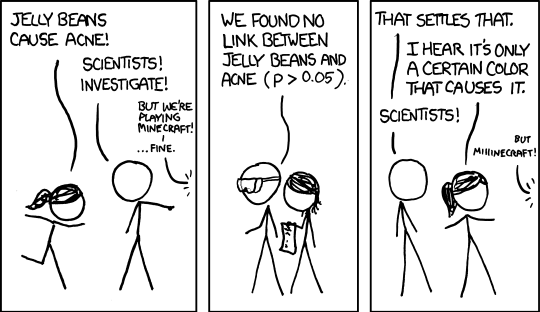
\includegraphics[height=26mm]{images/xkcd-882-top}};
   \node[inner sep=0pt,draw=SoftGray,below=2mm of top] (news) {
\includegraphics[height=32mm]{images/xkcd-882-news}};
   \node[inner sep=0pt,draw=SoftGray,right=4mm of top.north east,anchor=north west] (grid) {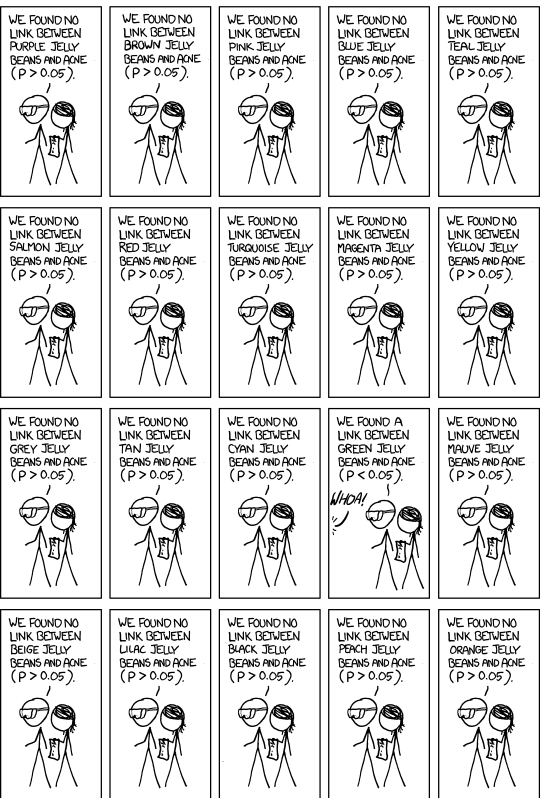
\includegraphics[height=60mm]{images/xkcd-882-grid}};
   \node[right=5mm of grid.north east,anchor=north west,text width=36mm,font=\small,align=left] {%
      Twenty colors tested at \(\alpha = 0.05\), one comes out significant, and only that one makes the news.\\[3mm]
      \textcolor{gray}{\footnotesize Comic\supercite{munroe2011significant} \link{https://xkcd.com/882/}{CC BY-NC 2.5}}};
\end{tikzpicture}
\ShowPerson{munroe}
\NoteRef{testing/twenty-jelly-beans}
\end{frame}

\begin{frame}{Multiple Testing}
\begin{tikzpicture}[
   Test/.style={circle,draw=SoftGray,fill=BackGray,minimum size=6mm,inner sep=0pt,font=\tiny},
   Hit/.style={Test,draw=Warn,fill=Warn!25,font=\tiny\sbseries},
]
   \foreach \i in {0,...,19} {
      \pgfmathtruncatemacro\col{mod(\i,5)}
      \pgfmathtruncatemacro\row{div(\i,5)}
      \node[Test] (t\i) at (\col*8mm,-\row*8mm) {};
   }
   \node[above=3mm,font=\small,align=center] at($(t0.north)!.5!(t4.north)$) {20 true null hypotheses, \(\alpha = 0.05\)};
   \onslide<2->{\node[Hit] at(t13) {.03};}
   \node[right=12mm,anchor=north west,text width=6.8cm,font=\footnotesize,align=left,visible on=<3->] (chance) at([yshift=4mm]t4.north east) {%
      Chance of at least one false positive\\(for independent tests):\\
      \(1 - (1 - 0.05)^{20} \approx \mrValueOf{round(1 - 0.95^20, 2)}\)};
   \node[below=2mm of chance.south west,anchor=north west,text width=6.8cm,font=\footnotesize,align=left,visible on=<4->] (bonferroni) {%
      \textsb{Bonferroni}: test each at \(\alpha / m = 0.05 / 20 = 0.0025\).\supercite{dunn1961multiple}
      This keeps the family-wise error rate at most \(\alpha\), at the cost of power.};
\end{tikzpicture}
\ShowPerson{bonferroni}
\Stage[14mm]{Model}
\NoteRef{testing/multiple-testing}
\end{frame}


\begin{frame}[label=plot-multiple-tests]{Correcting for Many Tests}
\centering
\begin{tikzpicture}
   \node[Plot] (plot) at (0,0) {\includegraphics[width=6.6cm]{multiple-tests}};
   \node[right=6mm,anchor=north west,text width=5.6cm,font=\small,align=left] (fwer) at(plot.north east) {%
      \textsb{Hardly ever a single false positive}\\
      \textcolor{gray}{\footnotesize family-wise error rate (FWER)}\\[1mm]
      \textsb{Holm}:\supercite{holm1979sequential} sort the \(p\)-values, compare with \(\alpha/m\), \(\alpha/(m-1)\), \dots, and stop at the first miss. At least as powerful as Bonferroni\supercite{dunn1961multiple}};
   \node[below=4mm of fwer.south west,anchor=north west,text width=5.6cm,font=\small,align=left,visible on=<2->] (fdr) {%
      \textsb{Few false positives among many findings}\\
      \textcolor{gray}{\footnotesize false discovery rate (FDR)}\\[1mm]
      \textsb{Benjamini--Hochberg}:\supercite{benjamini1995fdr} compare the \(k\)-th smallest \(p\) with \(k\alpha/m\). Everything up to the last hit counts};
   \node[below=3mm of plot.south west,anchor=north west,text width=6.4cm,font=\footnotesize,visible on=<3->] {%
      \bR{p.adjust(}\NotShown{pvals}{p}\kern-.25em\bR{, method = "holm")}\\\bR{p.adjust(}\NotShown{pvalsb}{p}\kern-.25em\bR{, method = "BH")}\\[.5mm]\textcolor{gray}{\texttt{p}: all your \(p\)-values}};
\end{tikzpicture}
\PlotCode{multiple-tests}
\Stage{Model}
\NoteRef{testing/plot-multiple-tests}
\NoteBoard{\begin{tabular}{@{}lccccl@{}}
   sorted \(p\)-values, \(m = 4\) & 0.001 & 0.015 & 0.030 & 0.040 & \\
   Bonferroni, always \(0.05/4\) & \BoardHit{0.0125} & 0.0125 & 0.0125 & 0.0125 & 1 significant\\
   Holm, \(0.05/4\), \(0.05/3\), \dots & \BoardHit{0.0125} & \BoardHit{0.0167} & 0.025 & stop & 2 significant\\
   Benjamini--Hochberg, \(k \cdot 0.05/4\) & \BoardHit{0.0125} & \BoardHit{0.025} & \BoardHit{0.0375} & \BoardHit{0.05} & 4 significant
\end{tabular}}
\end{frame}

\begin{frame}{The Garden of Forking Paths}
\begin{tikzpicture}[
   Choice/.style={Pill=BaseGray!70,font=\scriptsize\sbseries},
   Leaf/.style={font=\scriptsize,text=gray,inner sep=2pt,text height=1.6ex,text depth=.45ex},
   Lucky/.style={Pill=Warn,font=\scriptsize\sbseries,inner sep=2pt},
   level distance=15mm,
   level 1/.style={sibling distance=42mm},
   level 2/.style={sibling distance=21mm},
   level 3/.style={sibling distance=10.5mm},
   edge from parent path={(\tikzparentnode.south) -- ++(0,-4mm) -| (\tikzchildnode.north)},
   edge from parent/.style={draw,SoftGray,thick,rounded corners=3pt},
   grow=down,
]
   \node[Choice] (root) {raw data}
      child {node[Choice] {all rows}
         child {node[Choice] {raw}
            child {node[Leaf] {.21}}
            child {node[Leaf] {.34}}}
         child {node[Choice] {log}
            child {node[Leaf] {.12}}
            child {node[Leaf] {.08}}}}
      child {node[Choice] {no outliers}
         child {node[Choice] {raw}
            child {node[Leaf] {.09}}
            child {node[Leaf] {.06}}}
         child {node[Choice] {log}
            child {node[Leaf] {.11}}
            child {node[Lucky,visible on=<2->] (lucky) {.04}}}};
   \node[below=.5mm,font=\tiny\sbseries,text=Warn,visible on=<2->] at(lucky.south) {published};
   \foreach \level/\what in {1/subset,2/transform,3/{test: \(p\)}} \node[anchor=east,font=\scriptsize,gray] at(-4.4,-\level*15mm) {\what};
   \node[right=7mm,anchor=north west,text width=4cm,font=\small,align=left,visible on=<3->] (hack) at([yshift=2mm]root.north -| lucky.east) {%
      \textsb{\(p\)-hacking}: trying analyses until one is significant.\supercite{simmons2011falsepositive,head2015phacking}};
   \node[below=2.5mm of hack.south west,anchor=north west,text width=4cm,font=\small,align=left,visible on=<4->] (hark) {%
      \textsb{HARKing}: hypothesizing after the results.\supercite{kerr1998harking}};
   \node[below=2.5mm of hark.south west,anchor=north west,text width=4cm,font=\small,align=left,visible on=<5->] (fork) {%
      Each data-driven choice could go another way.\supercite{gelman2014forking}};
   \node[below=2.5mm of fork.south west,anchor=north west,text width=4cm,font=\small,align=left,visible on=<6->] {%
      \textcolor{plotblue}{\sbseries Remedies}: preregister, script, report all.\supercite{munafo2017manifesto}};
\end{tikzpicture}
\KeyMessage<6->{Write down the analysis before you see the results, and report all of it.}
\ShowPerson{borges}
\Stage[14mm]{Model,Communicate}
\NoteRef{testing/the-garden-of-forking-paths}
\end{frame}

\begin{frame}[label=plot-benchmark,optional]{Benchmarking a Tool}
Compare the simulated run times of two tools, A and B, on the same input:\supercite{berger2018checklist,ralph2021standards}\\[2mm]
\begin{columns}[c,onlytextwidth]
   \begin{column}{.42\textwidth}
      \centering
      \begin{tikzpicture}
         \node[Plot] (plot) {\includegraphics[width=5cm]{benchmark-1}};
         \node[below=1mm,Note,font=\small] at(plot.south) {one process of tool A};
      \end{tikzpicture}
   \end{column}
   \begin{column}{.54\textwidth}
      \small
      \begin{itemize}
         \item<2-> Repeat: fresh processes, several runs each\supercite{kalibera2013rigorous}
         \item<3-> Discard the warm-up, check for a steady state\supercite{barrett2017warmup}
         \item<4-> Quiet machine: no load, fixed CPU frequency
      \end{itemize}
   \end{column}
\end{columns}
\PinguSays<5->{Even the link order can shift run times by percents!\supercite{mytkowicz2009wrong}}
\PlotCode{benchmark}
\Stage{Model}
\NoteRef{testing/plot-benchmark}
\end{frame}

\begin{frame}[fragile,label=comparing-tools,optional]{Comparing Two Tools}
\begin{columns}[c,onlytextwidth]
   \begin{column}{.3\textwidth}
      \centering
      \begin{tikzpicture}
         \node[Plot] (plot) {\includegraphics[width=3.4cm]{benchmark-2}};
         \node[below=1mm,Note,font=\small,text width=3.6cm,align=center] at(plot.south) {one point per process};
      \end{tikzpicture}
   \end{column}
   \begin{column}{.66\textwidth}
\footnotesize
\begin{minted}[escapeinside={!*}{*!},mrprefix={library(dplyr); library(tidyr); set.seed(7); runs <- expand_grid(tool = c('A', 'B'), process = 1:10, iteration = 1:30) |> mutate(level = rep(rnorm(20, 0, 3), each = 30), time = ifelse(tool == 'A', 100, 94) + level + 60 * exp(-(iteration - 1) / 3) + rnorm(n(), 0, 1.5)); steady <- runs |> filter(iteration > 10) |> summarize(time = mean(time), .by = c(tool, process))}]{R}
a <- !*\textcolor{NotShownGray}{steady}\NotShownAfter{steady}{steady}*!$time[!*\textcolor{NotShownGray}{steady}\NotShownAfter{steadyb}{steady}*!$tool == "A"]
b <- !*\textcolor{NotShownGray}{steady}\NotShownAfter{steadyc}{steady}*!$time[!*\textcolor{NotShownGray}{steady}\NotShownAfter{steadyd}{steady}*!$tool == "B"]
median(b) / median(a)     # 0.96: here B needs 4 % less
wilcox.test(a, b)$p.value # 0.035
mean(outer(a, b, ">"))    # A12 = 0.78: A slower
\end{minted}
      \small
      \begin{itemize}
         \item<2-> \textsb{One value per process}: runs inside a process depend on each other, so average them first\supercite{georges2007rigorous}
         \item<3-> \textsb{Ranks} for skewed run times: \bR{wilcox.test()} and \(\hat A_{12}\)\supercite{arcuri2014hitchhiker,vargha2000critique}\\
            {\footnotesize\color{gray}\(\hat A_{12}\): the chance that a process of A is slower than one of B; 0.5: neither tends to win}
      \end{itemize}
   \end{column}
\end{columns}
\VarNote[north]{ns-steady}{(34mm,3mm)}{one row per process}
\PlotCode{benchmark}
\KeyMessage<4->{Report how much faster, and how often.\supercite{berger2018checklist,ralph2021standards}}
\Stage{Model,Communicate}
\NoteRef{testing/comparing-tools}
\end{frame}

% the urls contain slashes, so the \foreach list names them by key
\csdef{check@sigplan}{https://www.sigplan.org/Resources/EmpiricalEvaluation/}
\csdef{check@sigsoft}{https://www2.sigsoft.org/EmpiricalStandards/}
\csdef{check@hoefler}{https://doi.org/10.1145/2807591.2807644}
\csdef{check@artifacts}{https://www.acm.org/publications/policies/artifact-review-and-badging-current}
\begin{frame}{Checklists for Empirical Evaluations}
\centering
\vspace*{4mm}
\begin{tikzpicture}[
   Gallery/.style={Card,align=center,text width=26mm,anchor=north,font=\scriptsize},
]
   \foreach[count=\i] \key/\name/\what in {
      sigplan/SIGPLAN Guidelines\supercite{berger2018checklist}/{claims, baselines, benchmarks, analysis, presentation},
      sigsoft/SIGSOFT Empirical Standards\supercite{ralph2021standards}/{what reviewers expect, per kind of study},
      hoefler/Twelve Rules\supercite{hoefler2015benchmarking}/{for reporting performance results},
      artifacts/Artifact Evaluation/{badges for available, functional, and reproduced artifacts}%
   } {
      \node[Gallery,visible on=<\i->,href node=\csuse{check@\key}] at({(\i-1)*32mm},0)
         {\Qr[PartTint]{19mm}{\csuse{check@\key}}\\[2mm]\parbox[t][7mm][t]{26mm}{\centering\textsb{\name}}\\[1mm]
          \parbox[t][11mm][t]{26mm}{\centering\textcolor{gray}{\what}}};
   }
\end{tikzpicture}
\KeyMessage<5->{Always consult checklists!}
\NoteRef{testing/checklists-for-empirical-evaluations}
\end{frame}

\NextNoteRef{testing/takeaways-1}
\Takeaways[Testing]{
   \Learning{check-square-o}{Plan the test and \(n\) first}{Decided after seeing \(p\)? Fine, but report it as exploratory.}
   \Learning{arrows-h}{Report effect, interval, and \(n\)}{How large, how certain, from how much data, and what it means.}
   \Learning{percent}{Read \(p\) correctly}{It is not the chance that \(H_0\) is true. It says how surprising the data would be without an effect.}
   \Learning{code-fork}{Count every test}{Many tests make false hits likely. Correct with Holm, report all.}
}
